\documentclass[10pt]{article}

\usepackage[margin=3cm]{geometry}
\usepackage{amsmath}
\usepackage{amsfonts}
\usepackage{amssymb}
\usepackage{amscd}
\usepackage{standalone}
\usepackage{float}
\usepackage{color}
\usepackage[shortlabels]{enumitem}
\usepackage{graphicx}
\usepackage{caption}
\usepackage[ngerman]{babel}
\usepackage{lscape}
\usepackage{cancel}
\usepackage{dirtytalk}

\graphicspath{ {./images/} }

\begin{document}
\begin{titlepage}
    \centering
    {\scshape\LARGE Hochschule für Technik und Wirtschaft Dresden \par}
    \vspace{1cm}
    {\scshape\Large Softwaresystem \glqq GPS-Track-App\grqq\par}
    \vspace{1.5cm}
    {\huge\bfseries Projektbericht\par}
    \vspace{2cm}
    {\Large\itshape Raphael Neubert, Alex Schechtel, Aleksandr Pronin, Quang Duy Pham, Tom Nicolai, Ludwig Schönthier\par}
    \vfill
    \vfill
    \begin{minipage}{0.3\textwidth}
        Themensteller:\\
        Coach:\\
        Verantwortlicher HSL:\\
        Projektzeitraum:
    \end{minipage}
    \begin{minipage}{0.4\textwidth}
        Prof. Dr.-Ing. Mario Neugebauer\\
        Dipl.-Inf. (FH) Christoph Zirkelbach\\
        Prof. Dr.-Ing. Jürgen Anke\\
        11.2021 - 07.2022
    \end{minipage}
    \vfill
\begin{table}[H]
    \begin{tabular}{llllll}
    \textbf{Vorname} & \textbf{Nachname} & \textbf{Matrikelnr.} & \textbf{Kürzel} &  &  \\
    Aleksandr        & Pronin            & 48405                & AP              &  &  \\
    Alex             & Schechtel         & 49662                & AS              &  &  \\
    Quang Duy        & Pham              &                      & QDP             &  &  \\
    Raphael          & Neubert           &                      & RN              &  &  \\
    Ludwig           & Schönthier        &                      & LS              &  &
    \end{tabular}
    \centering
\end{table}
\vfill

    {\large \today\par}
\end{titlepage}
\tableofcontents
\newpage
\abstract{
    Im Folgenden wollen wir unsere Arbeit am Projekt \say{GPS-Track-App} erläutern.
    Wir wollen dabei unsere Vorgehensweise beschreiben und über technische sowie projektorganisatorische Entscheidungen
    reflektieren. Dabei gehen wir nicht nur auf die Inhalte ein, die gut liefen, sondern beschreiben auch die 
    aufgetretenen Probleme.
}

\section{Projektplanung}
\subsection{Aufgabenstellung [AS]}
    Im Rahmen unserer Projektarbeit im Modul \say{Software Engineering} hat Prof. Mario Neugebauer uns die Möglichkeit gegeben,
    eine Smartphone App zu entwickeln, welche das erstellen von GPS-Tracks für einen mobilen 
    Roboter ermöglicht. Dies hat den Hintergrund, dass die meisten GPS-Track Apps sehr unflexibel sind und es daher nicht 
    möglich ist, Strecken auf Gegebenheiten des Roboters anzupassen. Das Hauptziel unserer Projektes war es also, eine App zu entwickeln, 
    welche Strecken des Roboters aufnimmt, die er optimal verarbeiten und umsetzen kann.
    Dabei mussten wir für jede implementierte Funktionalität,
    eine angenehme und einfach zu verstehende Darstellungsform für die App finden.
    Es sollte möglich sein die aufgenommenen GPS-Tracks abzuspeichern und in der App aufzulisten.
    Außerdem sollte man auf einen Server die GPS-Tracks hochladen oder auch herunterladen können.
    Ebenso sollte es die Option geben, die GPS-Tracks nach dem abspeichern noch zu bearbeiten und dabei spezielle Punkte (special points of interests) 
    hinzuzufügen, sowie auch Punkte des aufegnommenen Weges zu verändern/verschieben.
    Bei der Aufnahme eines GPS-Tracks war es außerdem wichtig, die Genauigkeit des GPS-Signals so hoch wie möglich zu halten. 
\subsection{Auftraggeber [AP]}
    Die Rolle des Product Owners und Auftraggebers hat Herr Prof. Mario Neugebauer. Die Lehrgebiete von Prof. Neugebauer
    reichen von Programmier- und Datenbankgrundlagen bis hin zu mobilen Systemen und Kommunikationstechnik in 
    mobilen Netzen. Als Product Owner stand er in regelmäßigem Kontakt mit unserem Team, unterstützte uns und
    bewertete die Leistung unseres Teams am Ende der Iteration. Er verfügt über genügend Erfahrung und Wissen,
    um als technischer Ansprechpartner für das Team zu fungieren. Die Zusammenarbeit mit ihm war ein entscheidender Teil 
    unseres Projekts, und sie hat sich als sehr erfolgreich erwiesen.

\subsection{Ausgangssituation [RN], [AS]}
\subsubsection{Softwareengineering-I}
Zu Beginn des Projektes waren wir zu acht. Darunter sechs Informatiker und zwei Wirtschaftsingenieure.
Das Projekt war eine Neuentwicklung. Es gab keinerlei bestehenden Strukturen oder Code. Dies hatte den Vorteil, dass wir
selbst alles Planen konnten und nicht sehr stark an die Entscheidungen von anderen gebunden waren. So konnten wir
selbst die zu verwendenden Technologien, z. B. die Frameworks und Programmiersprachen festlegen und mussten dabei
nur auf die Wünsche des Themenstellers achten. Dies machte es uns natürlich nicht nur leichter, denn auch
hier galt \say{With great power comes great responsibility.}. Wir mussten also sehr viel Zeit in Recherche stecken um
feststellen zu können, ob mit den, von uns ausgewählten Technologien die Funktionalitäten überhaupt implementierbar sind.\par
\medskip
Am Anfang des Projektes fehlte uns vor allem eines, Erfahrung. Erfahrung sowohl in der Verwendung der Technologien
aber viel mehr noch, Erfahrung in der Teamarbeit und der Organisation eines solchen Softwareprojektes.
Dies wurde uns vor allem am Ende von Softwareengineering-I klar, als wir nochmal das Abgabedokument durchschauten
und feststellten, wie ineffizient unsere Arbeit am Anfang war.

\subsubsection{Softwareengineering-II}
Am Ende des Moduls SE1 hatten wir einen umfassenden
Überblick in das System und den funktionalen Anforderungen gewonnen. 
Wir hatten jetzt auch schon den Code vom Prototyp. Viel wichtiger aber, wir hatten die Erfahrung und das Wissen, was
wir beides bei der Erstellung des Prototyps erlangt hatten. Somit war der Start in Softwareengineering-II wesentlich
angenehmer als der in Softwareengineering-I.\par
\medskip
Die zwei Mitglieder aus dem Studiengang Wirtschaftsingenieurwesen, verabschiedeten 
sich am Ende des SE1 Projektes.
Außerdem verließ ein weiteres Mitglied die Gruppe. Somit verkleinerte sich unsere Gruppe von acht Mitgliedern,
auf fünf. Jedoch bekamen wir aufgrund unserer geringen Kapazität, 
gegenüber anderen Gruppen ein Ersatzmitglied (Aleksandr Pronin). \par 
\medskip
 Die gute Note, die die Wirtschaftsingenieure erhalten hatten, gab auch den
Rest des Teams viel Motivation und so starteten wir in das Modul mit dem Vorsatz schon am Anfang des Semesters möglichst
viel fertig zu bekommen, um Stress am Ende wenn noch andere Belegarbeiten dazukommen zu vermeiden.
Im ersten Meeting brachten wir alle Mitglieder nochmal auf den selben Informationsstand, 
über die Aufgabenstellung und den Fortschritt. 
Außerdem überprüften wir unsere grobe Rollenverteilung und verteilten die Aufgabenbereiche 
(Server u. App implementierung, Analyst, Tester etc.)
auf die Mitglieder auf. Somit hatten wir alle Voraussetzungen für einen guten Start in das laufende Projekt in SE2.


\subsection{Rollenverteilung [AP], [RN]}
    Die Rollen im Team waren nicht streng verteilt. Jeder war in seinem Bereich und entsprechend seinen Kompetenzen an 
    dem Projekt beteiligt. Im Verlaufe des Projektes entstand von alleine eine Art Zuordnung von Fachgebiet und Person.
    Zum Beispiel war am Ende Aleksandr Pronin für die Entwicklung und technischen Lösungen für den Client-Server-Teil verantwortlich 
    und Alex Schechtel für UI-relevante Dinge zuständig. Die folgenden Tabellen zeigen die, zu Beginn der jeweiligen Semester,
    ursprünglichen Rollenverteilungen.
\begin{table}[H]
    \begin{tabular}{|l|l|}
    \hline
    Anton  Peschel    & Projektleitung                                      \\ \hline
    Felix Reuß        & Analyst, Unterstützung Projektleitung               \\ \hline
    Ludwig Schönthier & Analyst,  Test                                      \\ \hline
    Richard Michel    & Any Role                                            \\ \hline
    Raphael Neubert   & Developer, Entwurf, stellvertretende Projektleitung \\ \hline
    Alex Schechtel    & Developer, Tester, Any Role                         \\ \hline
    Tom Nicolai       & Developer, Tester                                   \\ \hline
    Quang Duy Pham    & Tester, Entwurf                                     \\ \hline
    \end{tabular}
    \centering
    \caption{ursprüngliche Rollenverteilung Softwareengineering-I}
\end{table}
\begin{table}[H]
    \begin{tabular}{|l|l|}
    \hline
    Ludwig Schönthier & Analyst,  Projektleitung                                \\ \hline
    Raphael Neubert   & Projektleitung, Developer, Entwurf, Deployment Engineer \\ \hline
    Aleksandr Pronin  & Developer, Entwurf, Deployment Engineer                 \\ \hline
    Alex Schechtel    & Developer,  Any Role                                    \\ \hline
    Tom Nicolai       & Developer, Any Role                                     \\ \hline
    Quang Duy Pham    & Tester, Any Role                                        \\ \hline
    \end{tabular}
    \centering
    \caption{ursprüngliche Rollenverteilung Softwareengineering-II}
\end{table}
Wie in Tabelle 2 zu erkennen ist übernahmen in Softwareengineering-II Ludwig Schönthier und Raphael Neubert die 
Projektleitung. Damit dies möglich war, wurden die Projektleiteraufgaben zwischen den beiden aufgeteilt und auf eine 
ständige Kommunikation in der Projektleitung gesetzt.

\subsection{Kommunikation [RN]}
Durch die Pandemie bedingten Einschränkungen haben wir in \say{Softwareengineering-I} ausschließlich online kommuniziert. Später, in \say{Softwareengineering-II} war dies nicht mehr nötig. Da unser Team aus drei verschiedenen
Studiengängen und verschiedenen Jahrgängen bestand, war es durch die verschiedenen Stundenpläne und Nebenjobs 
schwer einen Termin zu finden an dem alle an der HTW sind bzw. an die HTW kommen konnten. Da die online Kommunikation 
schon bei Softwareengineering-I sehr gut funktionierte, entschlossen wir uns bei Softwareengineering-II weiterhin online 
zu kommunizieren.\par
\medskip
Für die online-Kommunikation im Team verwendeten wir die Dienst \say{Element}. Element ähnelt vom Grundaufbau dem 
Dienst \say{Discord}, unterscheidet sich aber insofern, als das Element Open-Source und dezentralisiert ist.
In unserem Element-\say{Space} erstellten wir uns zunächst zwei Kanäle. Einen für allgemeine Besprechungen, 
einen für  Programmierungs- bzw. Implementierungsspezifische Konversationen. Später im Projekt merkten wir, das 
es oft vorkam, das wichtige Informationen im Chat in unwichtigere Informationen untergingen. Wir erstellten
daher noch einen dritten Kanal für alle wichtigen links und Termine.
Für die Meetings verwendeten wir zunächst die von Element bereitgestellte Gruppenanrufs-Funktion.
Nach einigen Updates von Element gab es allerdings einige Probleme bei den Gruppenanrufen. Wir entschlossen 
uns daher von nun an für unsere Meetings die Plattform \say{Jitsi} zu verwenden.
Jitsi ist eine Open-Source Konferenzservice mit dem man im Browser, 
ohne Anmeldung mit zwei Klicks eine Konferenz starten kann. Unsere Erfahrungen mit Jitsi waren ausschließlich positiv.\par
\medskip
Um eine stetige Kommunikation zu gewährleisten und somit die Chance für das Eintreten bzw. die Folgen
von fehlerhafte Kommunikation zu minimieren, trafen wir uns am Anfang des Projektes wöchentlich. Am Ende 
des Projektes war unsere Aufgabenverteilung und unser gegenseitiges Vertrauen gut genug, sodass wir, solange
eine stetige Kommunikation auch asynchron gewährleistet war, zwischen Meetings auch mal zwei Wochen Platz lassen konnten.\par
\medskip
Während unsere Meetings zunächst sehr unkoordiniert abliefen, ergab sich mit der Zeit eine immer besser werdende 
Meetingstruktur. Anfangs haben wir für jedes Meeting sehr aufwändige Protokolle geschrieben. Nach einer Weile stellten 
wir fest das kaum jemand die Protokolle las und uns daher keinen Mehrwert gab. Um einen Ausgleich zwischen 
investierter Zeit und Mehrwert zu bekommen, entschieden wir uns, nur noch die Treffen mit dem Themensteller oder dem Coach
zu protokollieren und in dem Fall, dass jemand an einem Meeting nicht teilnehmen kann, wir uns im Nachhinein mit der 
Person in Verbindung setzen und ihr kurz das Meeting zusammenfassen. Eine weitere Verbesserung erzielten wir dadurch
das wir anfingen das jeder am Anfang des Meetings kurz zeigte, was er in der letzten Zeit gemacht hatte.
Dies wirkte sich auf den allgemeinen Überblick des Teams, aber auch auf die Motivation der einzelnen Personen positiv aus.
Es gab noch kleine weitere Änderungen, die sich positiv auf die Meetings ausgewirkt haben. Neben den 
durch Änderungen ausgelösten diskreten Verbesserungen war aber auch eine, durch den Zuwachs an allgemeiner 
Erfahrung und Kompetenz ausgelöste stetige Verbesserung bemerkbar. Die Früchte der Verbesserungen waren unter anderen 
ein besseren Überblick den jedes Teammitglied über das Projekt hatte, jeder wusste nach dem Meeting genau, was er 
zu erledigen hatte, die Meeting Zeit wurde effizienter genutzt so das in weniger Zeit
mehr Informationen ausgetauscht werden konnten.
\par
\medskip

Am Ende unterteilten sich die Meetings meistens in vier Teile. Als Erstes haben wir immer über die in Ergebnisse
seit dem letzten Meeting gesprochen. Wie bereits erwähnt geschah dies oft so, das die einzelnen Teilnehmer 
kurz ihre fortschritte erklärten bzw. vorführten.  Danach besprachen wir die grobe weitere Planung. Dazu zählte die 
Überprüfung ob wir uns im Zeitplan befinden, die Priorisierung bzw. das Umpriorisieren von Funktionalitäten und die 
Planung von Meetings mit dem Themensteller oder Coach. Als Drittes setzten wir die Planung der aktuellen Funktionalitäten 
fort und erstellten Issues für die Weiterentwicklung. Im letzten Teil des Meetings teilten wir dann die Issues 
den Teammitgliedern zu. Dabei konnte es auch vorkommen, dass wir niedrig priorisierte Issues niemanden zuteilten, sondern 
diese, falls jemand schon schneller als erwartet mit seinen Issues fertig war, dieser Person zugewiesen wurde.\par
\medskip
Um Zeitverschwendung zu vermeiden planten wir die Meetings mit dem Themensteller oder dem Coach nur nach Bedarf.
Wir schrieben uns unsere fragen immer auf und sobald genug zusammengekommen waren bzw. eine Frage sehr 
wichtig war, planten wir ein Meeting. Für die Besprechung von kleinen, wichtigen Entscheidungen,
die schnell getroffen werden mussten war oft auch eine kurze Mail an den Themensteller ausreichend.
Während wir bei Softwareengineering-I häufig Meetings mit unserem Coach hatten, reduzierte sich die Anzahl
bei Softwareengineering-II stark. Dies war vor allem der Tatsache geschuldet das wir uns mehr auf die Entwicklung
der eigentlichen Software konzentrierten aber auch der Tatsache das wir
in unserem arbeiten viel sicherer geworden sind und dadurch weniger Fragen auftraten.
Die Meetings sowohl mit dem Themensteller als auch mit dem Coach empfanden wir immer als sehr sinnvoll. Meist 
trafen wir uns direkt nach dem Meeting, um die vorgeschlagenen dinge in Issues zu überführen die wir dann später 
umsetzten.\par 
\medskip 
Perfekt waren unsere Meetings am Ende aber noch lange nicht. Ein Problem was wir zum Beispiel nur vermindern aber 
noch nicht komplett lösen konnten war das, sich im Meeting beschränken auf Konversationen, die möglichst alle betreffen.
Zum Beispiel haben wir manchmal sehr detailliert über die Serversynchronisation gesprochen und das, obwohl an der 
Entwicklung der Synchronisation nur zwei Personen beteiligt waren. Solche Situationen entstanden unbewusst und 
wirkte sich, für alle am detaillierten Thema unbeteiligten negativ auf die Qualität des Meetings aus.

\subsection{Techniken/Praktiken}
\subsubsection{Git/GitHub [RN]}
Zur Entwicklung verwendeten wir Git und als Host GitHub. In unserem Team kannten sich anfangs nur zwei von acht Personen
mit Git aus. Wir passten daher die Komplexität unseres GitHub-Workflows dem Stand der Praktika an. Zum Beispiel
verwendeten wir erst mehrere Branches nachdem Branching im Praktikum behandelt wurden. Unsere GitHub-Workflows haben
wir im Verlauf des Projektes sehr häufig angepasst und verbessert.\par
\medskip
Von Anfang an verwendeten wir Issues zur Planung kleiner Aufgaben. Nach einer Weile merkten wir, dass es sinnvoll
ist, diese mittels eines Projektboards zu organisieren. Wir erstellten daraufhin ein Projektboard mit vier Spalten.
Die Spalte \say{Icebox} für Issues die noch niemanden zugewiesen wurden, die Spalte \say{Assigned} für Issues die
zwar zugewiesen, aber noch nicht in Bearbeitung waren, die Spalte \say{In Progress} für Issues die sowohl zugewiesen
als auch in Bearbeitung sind, und die Spalte \say{Done} für Issues deren Bearbeitung abgeschlossen ist.
Wir verwendeten dieses Projektboard für mehrere Iterationen. Als das Projektboard aber immer voller wurde, entschlossen wir uns
von nun an für jede Iteration ein Projektboard zu erstellen. Im Verlaufe des Projektes versuchten wir uns auch mal
an der Verwendung eines komplizierteren Projektboards mit Pull-Requests und Reviews, merkten aber schnell, dass
für den Umfang unseres Projektes, mit dieser Methode, Zeit und Nutzen in keinem guten Verhältnis standen.
Wir können uns allerdings vorstellen, dass die Verwendung eines solchen Projektboards für umfangreichere Projekte
sinnvoll ist. Am Ende verwendeten wir primitive 3 Spalten Projektboards mit den Spalten \say{To do}, \say{Assigned} und
\say{Done}, da wir feststellten, dass wir von der Spalte \say{In Progress} keinen Mehrwert erhielten und es aufwendig
war, jedesmal bevor man mit der Arbeit anfangen konnte eine Änderung am Board vornehmen zu müssen. Die Projektboards
automatisierten wir so, dass beim Schließen eines Issues, sei es manuell oder durch Referenzierung des Issues in
der Commit-message, dieser Automatisch in die Spalte \say{Done} verschoben wurde.\par
\medskip
Wie bereits erwähnt verwendeten wir zunächst nur einen Branch. Für alles was nur mit Dokumentation und Anforderungsanalyse
zu tun hatte, funktionierte dies problemlos. Bei der Entwicklung hingegen gab es ab und zu kleine Probleme.
Zum Beispiel ist es mal vorgekommen, dass wir kurz vor einem Meeting mit dem Themensteller feststellen mussten, dass
die App nicht mehr kompilierte. Gelöst haben wir das Problem in dem wir einen \say{checkout} zu einer älteren Version
gemacht haben und nach dem Meeting den Fehler gesucht und gelöst haben, aber dies brachte uns auf eine Idee.
Wir wollten von nun an mehrere Branches verwenden und für diese, sowie deren Interaktion verschiedene Regeln aufstellen.
Eine Regel war zum Beispiel, dass die sich auf dem Hauptbranch befindende Version immer erfolgreich kompilieren
und keine größeren Bugs beinhalten muss. Wir erstellten den Branch \say{dev} auf dem wir von jetzt an entwickelten.
Immer wenn eine Funktionalität fertig entwickelt und ausreichen gut getestet war, haben wir den \say{dev}-Branch in
unseren Hauptbranch gemerged und somit den Hauptbranch aktualisiert. Später versuchten wir für jedes Feature einen
eigenen Branch zu erstellen und nach Fertigstellung diesen in den \say{dev}-Branch zu mergen. Wir mussten aber feststellen
das dies zum einen sehr aufwendig war, oft aber auch kaum möglich, da es Abhängigkeiten zwischen den Features gab,
die erst bei der Entwicklung auffielen. Wir entschlossen uns daher nur für große, ganz klar unabhängige Features
weitere Branches zu erstellen und behielten dieses Branching-Modell bis zum Ende des Projektes bei.

\subsubsection{Iterationen [RN]}
Ein weiterer Faktor, der sich im Verlauf des Projektes stark geändert hat, ist die Planung der Iterationen.
Anfangs arbeiteten wir noch nicht nach Iterationen. Erst nach Gesprächen mit unserem Coach merkten wir aber
wie wichtig Iterationen sind. Wir begannen also in Iterationen zu arbeiten. Die ersten Iterationen lang
betrachteten wir Iterationen als ein ausschließlich zeitlichen Rahmen und starteten jede Woche eine neue Iteration.
Vor allem als die eigentliche Entwicklung begann, merkten wir, dass dies nicht sinnvoll ist, vor allem
da wir alle unerledigten Issues einfach nur in die nächste Iteration schoben. Zu diesem Zeitpunkt schrieben wir
die Iterationspläne oft erst nach der Beendigung der Iteration und füllten den Punkt \say{Wesentliche Ziele} aus in dem
wir schauten, was wir fertig bekommen hatten und nicht so wie es eigentlich gedacht ist, vorher.
Als wir zu der Erkenntnis kamen, dass dies nicht viel Sinn ergibt, entschlossen wir uns von da an
die Iterationen nach konkreten Zielen, meist Funktionalitäten zu planen. Dies funktionierte zunächst ziemlich gut.
Es kam dadurch allerdings vor, dass die Iterationen sehr lang wurden.\par
\medskip
Durch den Fachaustausch zum Thema Projektmanagement wurde uns klar, dass wir unsere Iterationen noch nicht optimal planten.
Wir überarbeiteten unser Iterationsplanmodell ein letztes Mal. Wir kombinierten unser erstes und unser zweites Modell.
Unsere Iterationen bekamen wieder einen festen Zeitrahmen. Zusätzlich legten wir aber noch eine Funktionalität, oft
aber auch nur eine Teil-Funktionalität fest, die auf jeden Fall in dem Zeitrahmen erledigt werden konnte und dann auch wurde.
Wir hatten somit ein sehr gutes Iterationsplanmodell gefunden. Leider waren wir am Ende so auf die
Entwicklung fokussiert, dass wir unser eigentliches Iterationsplanmodell und die Iterationen selber etwas vergessen
haben. Wir sind uns aber sicher, dass wenn wir uns diszipliniert an unser Iterationsplanmodell gehalten hätten,
wir organisierter und effizienter unsere Ziele erreicht hätten.

\subsubsection{Alphas [LS]}
Da wir die Nutzung der Alpha States oft vergessen und allgemein unregelmäßig genutzt haben, hatte das Team das Gefühl, diese seien 
keine große Bereicherung. Der Fortschritt unseres Projekt wurde anhand unserer Iterationen innerhalb des GitHub Repositorys gut deutlich und die
Ausarbeitung spezieller Checklisten und Ziele erschien uns oft als zu viel Aufwand, der nicht dem Projektumfang entsprach. Innerhalb unseres Projektes
waren die Ziele und Meilensteine relativ klar erkenntlich und benötigten in unseren Augen keinerlei zusätzliche Dokumentation.

\subsubsection{\dq Compression based Programming\dq\,\,[RN]}
Mit \say{Compression based Programming} meinen wir einen Programmierstiel, der sich für uns als besonders gut 
herausgestellt hat. Dabei schrieben wir bei der Implementierung von Funktionalitäten, zunächst alles in eine einzige 
Methode. Erst dann fingen wir an uns Gedanken über die Strukturierung zu machen. Weil man zu diesem Zeitpunk bereits 
eine fertige Implementierung hatte, war eindeutig zu erkennen ob es Sinn machte Inhalte in eine 
eigene Klasse zu kapseln. Nach dieser Entscheidung galt es allen, in der Methode mehrfach verwendeten Code zu 
finden und in Methoden zu kapseln. Die ursprüngliche Methode wird dabei immer kleiner also kompressiert. 
Als nächstes lagerten wir alle Zustands-unabhängigen Zeilen Code in viele kleine Methoden aus, so dass jede Methode 
genau eine Aufgabe erfüllte. Dadurch wurde die ausgangs-Methode noch kleiner. Ziel dieses Programmierstieles ist 
es, Code möglichst gut wiederzuverwenden und eine Trennung zwischen Zustands verändernden und rein logischen Methoden
zu schaffen.\par 
\medskip 
Der Nachteil dieses Stiels war, dass es sehr viel Nacharbeit bedarf. Oft waren wir zu faul um diese Nacharbeit direkt 
nach der Implementierung einer Funktionalität durchzuführen.  Irgendwann fiel uns das meistens auf die Finger. 
Wir mussten dann durch mühseliges Refactoring dann im Nachhinein eine Struktur schaffen. Hätten wir immer direkt nach 
der Implementierung das Refactoring betrieben, dann hätten wir uns Zeit gespart und das Ergebnis währe besser gewesen.
Wir sind dennoch von unserer Strategie überzeugt, denn es ist fast ausgeschlossen ohne die Lösung zu kennen auf Anhieb 
perfekten Code zu schreiben. Außerdem beeinflusst das Trennen von Zustands verändernden und rein logischen Methoden, 
die Nachvollziehbarkeit positiv. 
\subsubsection{Risikoanalyse}
Wie wir die Risikoanalyse durchgeführt haben wird im Kapitel \say{Projektdurchführung} in der Inception-Phase beschrieben.
\subsubsection{Testing}
Unsere Umsetzung des Testens wird im Kapitel \say{Projektdurchführung} in der Elaboration, Construction
und Transition-Phase sowie in der Testdokumentation beschrieben.

\newpage
\section{Projektdurchführung}
Im folgenden werden die vier Phasen unseres Projektes: Inception, Elaboration, Construction und Transition im Detail erklärt. Im Anhang des Dokuments befinden sich
weiterhin die Iterationspläne der Iterationen, welche der jeweiligen Phase zuzuordnen sind. Leider gibt es keine Pläne zu den Iterationen 1 und 2, da wir erst in der dritten
Iteration mit der Erstellung der Pläne begonnen haben.
\subsection{Phase: Inception [AS], [RN]}
(Iteration 1) \\
Die Inception Phase war die erste Phase des Projekts. Nachdem wir uns kennengelernt hatten, sprachen wir über
unsere verschiedenen Erfahrungsstände in der Softwareentwicklung und verteilten die Rollen entsprechend.
Anschließend planten wir ein Treffen
mit unserem Themensteller, in Vorbereitung schrieben wir dazu eine Liste mit allen Fragen, die uns zum Projekt einfielen.
Beim Treffen mit dem Themensteller besprachen wir ausgiebig das Projekt und notierten alle wichtigen Informationen
in einem Meetingprotokoll.\par
\medskip
Begonnen haben wir mit der Einrichtung der Projektumgebung. Da schon nach dem ersten Meeting klar war, dass es sich
um eine native Android-App handeln wird, installierten alle die in der Entwicklung tätig sein wollten, das IDE
\say{Android-Studio}. Ferner erstellten wir das GitHub-Repository und stellten sicher, dass jedes Teammitglied
Zugriffsrechte drauf hatte.\par
\medskip
Leider informierten wir uns nicht über die Inhalte der Phase, sondern arbeiten einfach drauflos.
So vergasen wir die Erarbeitung der Vision, was sich später noch rächen sollte.
Einer unserer ersten Schritte war die Erarbeitung der Use-Cases.
Wir trafen uns dafür im Team und besprachen die verschiedenen Anwendungsmöglichkeiten,
die unsere App bekommen sollte. Im Nachhinein stellten wir fest, dass schon hier, der durch das nicht
Erarbeiten der Vision fehlende Überblick zu merken war. So war es zum Beispiel einigen nicht klar, dass die
App mit den Robotern noch nichts direkt zu tun haben wird. Ein weiteres Problem war, dass wir uns unsicher waren
wie detailliert unsere Use-Cases sein sollten. Anfangs erstellten wir die Use-Cases sehr grob, dann sehr detailliert
und am Ende irgendwo dazwischen. Nach der Erstellung priorisierten wir noch die Use-Cases. Unseren Entwurf besprachen
wir dann mit unserem Coach und passten das Modell entsprechend des erhaltenen Feedbacks an. Unser
Themensteller war mit unserem Entwurf zufrieden, lediglich die Priorisierung passten wir noch an.\par
\medskip
Die Identifikation der Risiken erfolgte in einer kleinen Gruppe. Anschließend wurden die identifizierten Risiken aber
mit dem gesamten Team besprochen, eingeschätzt und ihnen entsprechende Gegenmaßnahmen zugeordnet.
Wir sind der Meinung, dass diese gemeinsame Risikobewertung allen
ein verbessertes Bewusstsein über möglich auftretende Probleme gab und dadurch auch den Workflow positiv beeinflusste.
Wir entschlossen daher die Risikobewertung vor jeder Iteration, weiterhin im Team durchzuführen. \par
\medskip
Wir machten uns in der Inception Phase auch schon erste Gedanken zur Architektur und den zu verwendenden Technologien.
Durch die Risikoanalyse war uns aber klar, dass eine falsche Wahl, fatale Folgen für das Projekt haben könnte.
Somit nahmen wir uns viel Zeit zum intensiven Recherchieren, um feststellen zu können, ob die Use-Cases mit den
verschiedenen Technologien umsetzbar sind. Weil außer der Recherche auch einiges Experimentieren notwendig war,
trafen wir einige Technologieentscheidungen erst in der Elaboration Phase.\par
\medskip
Das Lifecycle Objective: \say{Die Beteiligten sind sich darüber einig, was erreicht werden soll (Ziele sind
klar) und es ist technisch möglich und es ist ökonomisch sinnvoll} hatten wir durch das Versäumnis, die Vision
auszuarbeiten nicht leider vollständig erfüllt bevor wir in die Elaboration Phase gestartet sind.

\newpage
\subsection{Phase: Elaboration [RN]}
(Iteration 2, 3, 4)\\
Nach dem Abschluss der Inception-Phase begann die Elaboration Phase. Dass wir die Inception-Phase nicht optimal
beendet hatten, wussten wir zu diesem Zeitpunkt noch nicht, doch dies sollte sich bald ändern.\par
\medskip
Wir begannen mit der detaillierten Ausarbeitung der drei höchstpriorisieren Use-Cases. Die Ausarbeitung übernahmen
dabei einzelne Personen, wir besprachen die Ergebnisse aber in einem Projektmeeting. Dabei mussten wir leider feststellen,
dass es im Team immer noch Unklarheiten über den Umfang des Projektes gab. Diese Unklarheiten schienen unserem Coach
in einem Meeting aufgefallen zu sein, denn wir wurden explizit nach der Vision gefragt. Erst jetzt bemerkten wir,
dass diese noch fehlte. Wir pausierten also die Arbeit an den Use-Cases und erstellten die Vision. Nachdem wir die
Vision im Team besprochen hatten, war allen der Umfang des Projektes, sowie das eigentliche Ziel klar. Die Vision
ist uns ebenfalls am Anfang von Softwareengineering-II nützlich geworden, als Aleksandr Pronin unserm Team
beigetreten ist, und wir ihn auf die Vision verweisen konnten, die ihm Kontext zu unserer Arbeit gab.\par
\medskip
Nachdem wir nun endlich die Vision erstellt hatten, setzten wir die Arbeit an den Use-Cases fort.
Zunächst beschrieben wir alle textuell, merkten aber, dass es für einen der Use-Cases als sinnvoll erschien, ein UML-Aktivitätsdiagramm
zu verwenden.\par
\medskip
Parallel zur Arbeit an den funktionalen Anforderungen arbeiten wir auch an den
systemweiten Anforderungen im Sinne des FURPS+ Modells und an den zusätzlichen Anforderungen des Projektes.
Dabei standen wir im engen Kontakt mit unserem Themensteller. Wir machten leider auch hier einige Fehler.
Zum Beispiel stellten wir Anforderungen, deren Erfüllung nicht eindeutig überprüft werden konnte, oder wir
stellten Anforderungen, die uns einschränkten, aber nicht vom Themensteller oder vom Projekt zwingen gefordert waren.\par
\medskip
Um unser Vorhaben noch besser mit unserem Themensteller kommunizieren zu können, erstellten wir drei Wireframes
die verschiedene Teile unserer geplanten App darstellten. Das Resultat war ein sehr ertragreiches Meeting, bei dem
wir von unserem Themensteller sehr viele gute Ideen und Umsetzungsvorschläge erhielten. Die Verwendung von Wireframes
hat uns daher sehr überzeugt und wir nehmen uns vor, diese auch in zukünftigen Projekten zu verwenden.\par
\medskip
Neben der Anforderungsanalyse, beschäftigten wir uns auch intensiv mit der Wahl der Technologien.
Durch unsere Recherche während der Inception-Phase, kannten wir die verschiedenen Technologie-Kombinationen,
die für unsere Aufgabenstellung geeignet zu sein schienen. Jetzt galt es herauszufinden, welche davon die beste für uns
ist und ob mit dieser alle gewünschten Funktionalitäten implementierbar waren. Die Wahl der Programmiersprache,
sowie dem Framework für den Server war für uns leicht, den ein Teammitglied hatte bereits mit der Programmiersprache
Python sowie dem Framework Flask gearbeitet und war sich sicher, dass es für unsere Zwecke gut geeignet ist.
Bei der Programmiersprache für die App, mussten wir zwischen Java und Kotlin wählen, denn nur diese beiden Sprachen
erlauben eine naive Android-Entwicklung, die zwingend notwendig war, um komplexere Kartenmanipulation betreiben zu können.
Während Kotlin einige tolle Features hat, die Java nicht hat, hatte Java einen entscheidenden Vorteil.
Java, sowie die Verwendung der Android-SDK mit Java, ist viel besser dokumentiert als Kotlin.
Wir entschlossen uns aus diesem Grund für die Verwendung von Java, jedoch war diese Entscheidung keine kritische,
denn es ist möglich eine App in Java und Kotlin zu schreiben. Wir hätten also trotz unserer Entscheidung,
einzelne Klassen auch in Kotlin schreiben können, was wir aber nicht taten.

Jetzt blieb nur noch die Wahl der Bibliothek zur Arbeit mit Karten und Kartendaten. Dies stellte sich als die
schwerste Entscheidung heraus. Es gab bei dieser Wahl zwei Konkurrenten. Zum einen die offizielle
Maps-SDK von Google, zum anderen Osmdroid, eine Open-Source Ersetzung der Maps-SDK. Wir verbrachten viel Zeit
mit der Analyse beider und trafen dann (vorerst) eine Entscheidung. Wir entschlossen uns Osmdroid zu verwenden, weil es fast alle Funktionalitäten wie die Maps-SDK hatte, aber viel besser dokumentiert war. Des Weiteren
waren wir mit Osmdroid unabhängig von Google oder irgendeinen anderen Kartendatenanbieter, denn
Osmdroid ermöglicht die Verwendung von verschiedenen Kartendatenanbietern. Wir brauchten daher
keinerlei API-Schlüssel, weil wir uns die Kartendaten von einem freien Anbieter holten.
Der Hauptgrund war jedoch, dass Osmdroid Open-Source war. Im Nachhinein waren wir sehr froh über diese Entscheidung.
Wir haben oft in den Quellcode der Bibliothek geschaut, um herauszufinden, wie verschiedene Dinge funktionieren.
Außerdem standen uns auf der GitHub-Seite von Osmdroid 1206 Issues zur Verfügung von Personen, die ähnliche
Probleme wie wir hatten. Wir glauben, dass wir, falls wir die Maps-SDK verwendet hätten, im Projekt nicht so weit
gekommen wären und merken uns für die Zukunft uns immer die Open-Source Alternativen zu den offiziellen APIs
anzuschauen.\par
\medskip
Zu diesem Zeitpunkt wussten wir aber noch nicht, dass Osmdroid eine gute Wahl sein wird. Wie auch?
Osmdroid bot über 500 verschiedene Klassen an. Es war uns zu Beginn also nicht möglich einschätzen zu können,
ob alle Use-Cases, vor allem der Use-Case \say{GPS-Track bearbeiten} mit der Bibliothek implementierbar ist.
Wir entschlossen uns, genau dies durch die Entwicklung des Prototyps herauszufinden.\par
\medskip
Unser Prototyp erfüllte daher keinen einzigen Use-Case komplett, aber enthielt Elemente, die wir für die
Implementierung der wichtigsten Use-Cases brauchen sollten. Im Folgenden sind die im Prototyp implementierten Elemente
der wichtigsten Use-Cases, sowie die daraus gewonnenen Erkenntnisse beschrieben.
\begin{itemize}
\item \textbf{GPS-Track aufnehmen}\\
Wir implementierten das Anzeigen einer Karte, sowie des aktuellen Standorts.
Außerdem fügten wir erste UI-Elemente, z. B. einen Button zum Starten einer Aufnahme und einen Button
zum Zentrieren der Karte auf den aktuellen Standort hinzu. Um dies zu bewältigen, beschäftigten
wir uns intensiv mit der Erstellung des \say{Boilerplate}-Codes, der nötig war, um eine Karte anzeigen
zu können. Zudem beschäftigten wir uns mit dem Managen von Berechtigungen,
die nötig waren, um Zugriff auf den Speicher (für Karten-Cache) und
den GPS-Sensoren (Standort) zu erlangen, sowie den verschiedenen Möglichkeiten auf Positionsdaten zuzugreifen.
Wir erlangten auch Kenntnisse über die Interaktion von UI-Elementen und Code, denn wir implementierten den
Zentrieren-Button so, dass er ausgeblendet wurde, solange die Karte auf den Standort zentriert war.
\item \textbf{GPS-Track auflisten}\\
Wir implementierten eine zweite Aktivität (Seite), die dem Auflisten der gespeicherten GPS-Tracks dienen
sollte. Dort beschäftigten wir uns mit der iterativen Erzeugung von Listenelementen sowie der Erzeugung
eines Untermenüs beim Klick eines Listenelements. Die Interaktion mit dem Dateisystem hatten wir nur mithilfe
von Konsolen-Outputs getestet. Wir erlangten hier weitere UI-Kenntnisse sowie die von der Android-SDK gegebenen
Möglichkeiten, mit dem Dateisystem zu interagieren.
\item \textbf{GPS-Track auf Karte anzeigen}\\
Wir versuchten Pfade auf der Karte anzuzeigen. Dies gelang uns unter der Verwendung von Polylines.
Unsere Tests löschten bzw. kommentierten wir vor der Vorstellung des Prototyps aus, damit dieser möglichst
sauber und nicht so überladen erschien. Das Wissen bzw. die Erfahrung über/mit Polylines blieb aber.
\item \textbf{GPS-Track bearbeiten}\\
Hier beschäftigten wir uns vor allem mit Marken, welche wir auf der Karte platzierten.
Die wichtigste Erkenntnis aus unseren Tests mit Markern war, dass man für Marker die
Callback-Funktionen \say{onMarkerClick()} und noch viel wichtiger \say{onMarkerDrag()} implementieren konnte.
Diese wurden später für die Implementierung des Use-Cases sehr wichtig.
\end{itemize}

\newpage
Nachdem wir die Implementierung des Prototyps beendet hatten, waren wir uns sicher, dass
wir die Implementierung aller Use-Cases mit Osmdroid umsetzen konnten. Wir hatten somit eines der größten Risiken eliminiert.
Jetzt schrieben wir noch einen Testcase für den Prototyp und fertigten das Domainmodell an. Der Code des Prototyps war
sehr chaotisch und unstrukturiert. Die Anfertigung des Domainmodell gab uns Ideen, wie wir Dinge strukturieren könnten.
Diese setzten wir dann in Softwareengineering-II auch um.
Die restliche Zeit verbrachten wir mit der Verbesserung,
der für die Softwareengineering-I Abgabe notwendigen Dokumente.

\subsection{Phase: Construction [RN]}
(Iteration 5, 6, 7) \\
In der Construction Phase, welche am Anfang von Softwareengineering-II begann, galt es,
alle Hochpriorisieren Use-Cases vollständig zu implementieren und falls noch Zeit ist, auch
die niedriger priorisierten Use-Cases umzusetzen. Wir begannen mit einer Überarbeitung des Prototyps. Im Prototyp hatten 
wir bis dahin nur zwei Klassen mit sehr langen Methoden die viele verschiedene Dinge taten. Wir verwendeten 
die, durch das Domainmodell gewonnene Inspiration um Dinge in neue Klassen auszulagern. Auch die Methoden 
vereinfachten wir stark, mit dem Ziel, dass die meisten Methoden nur eine einzige Aufgabe besaßen.
Bis zu diesem Zeitpunkt waren nur zwei Teammitglieder am Prototyp involviert. Uns war aber klar, dass wir um möglichst 
viele Use-Cases erfüllen zu können, das Entwicklungsteam vergrößern müssen. Wir erklärten daher, allen bisher am Code 
unbeteiligten, unsere bisherigen Implementierungen und ließen genügend Zeit für die Einarbeitung.\par 
\medskip
Beim Erstellen der Issues mussten wir feststellen, dass es nicht möglich ist die Aufgaben so zu verteilen, dass 
alle gleichzeitig am gleichen Use-Cases arbeiten. 
Wir begannen also, uns entsprechend unserer Stärken in kleinere Gruppen zu unterteilen, wobei
es möglich war, dass eine Person zwei Gruppen angehörte. Dadurch ermöglichten 
wir eine parallele Bearbeitung der Funktionalitäten. Sobald ein Use-Case fertig implementiert war, informierten 
wir den Tester darüber. Dieser unternahm dann ein umfangreiches Testing und meldete uns alle gefundenen Fehler.
Falls wir zu diesem Zeitpunkt schon mit der Bearbeitung eines weiteren Use-Cases begonnen hatten, pausierten wir diese 
und behoben erstmal die Fehler des abgeschlossenen Use-Cases.
Im Folgenden wollen wir unser Vorgehen für die Implementierung der einzelnen 
Use-Cases beschreiben und auf entstandene Probleme, sowie deren Lösungen eingehen.

\paragraph{GPS-Track aufnehmen} \quad\\
An diesem Use-Cases waren 3 Teammitglieder beteiligt. Zunächst machten wir uns Gedanken über die Speicherung 
der GPS-Tracks. Wir recherchierten daher bezüglich der verschiedenen Dateiformate. Nach einiger Zeit merkten wir, 
dass es in einem Osmdroid Bonuspaket, Möglichkeiten gab, GPS-Tracks als KML-Datei zu exportieren. 
Dies gefiel uns, uns war aber auch die Wichtigkeit dieser Entscheidung bewusst. Deshalb nahmen wir Kontakt zu unserem 
Themensteller auf. Durch das Gespräch wurde uns klar, dass wenn auch komfortabel, KML nicht die richtige Entscheidung 
für Speichern von GPS-Tracks war, da es für die Verwaltung von wesentlich mehr Informationen, als die von uns benötigten,
gedacht ist. Zum Glück hatten wir uns vor dem Meeting schon über alternative Dateiformate informiert und so besprachen 
wir die anderen Dateiformate und trafen gemeinsam mit dem Themensteller die Entscheidung, das Format \say{GPX} zu verwenden,
weil es genau für Zwecke, wie die unseren gedacht war.\par 
\medskip
Weil es in Osmdroid leider keine Möglichkeit gab, GPS-Track-Daten als GPX zu exportieren und das Schreiben eines eigenen
GPX-Parsers zu aufwendig gewesen wäre, suchten wir im Internet nach einem passenden GPX-Parser. Die Suche 
stellte sich als schwerer als erwartet raus. Die erste Bibliothek, die wir versuchten war inkompatibel mit der 
für die App verwendeten Java Version. Die Zweite konnte GPX Dateien zwar parsen, jedoch gab es keine Möglichkeit unsere GPS-Track-Daten, als GPX zu exportieren. Die Dritte bestand all unsere Tests, wir waren uns aber mit der 
Lizenzierung unsicher und nahmen daher nochmal Kontakt zum Themensteller auf. Es stellte sich heraus die Lizenzen 
kompatibel sein sollten, somit hatten wir eine passende Bibliothek gefunden.\par 
\medskip 
Jetzt konnte die Arbeit beginnen. Wir teilten uns dabei so auf, dass einer sich mit dem Holen der Positionsdaten, 
einer mit dem Export und Import der GPX-Dateien, und einer mit den UI-relevanten Dingen beschäftigte. Bei der Entwicklung 
testeten wir die Funktionalität nur grob im Emulator und stellten fest, dass alles funktionierte.\par 
\medskip
Wir erklärten somit die Entwicklung des Use-Cases für abgeschlossen und informierten unseren Tester. 
Dieser erstellte einen Testfall und begann mit dem Testen, jedoch nicht nur im Emulator, sondern auch auf einem 
echten Gerät. Der Tester stellte fest, dass im Großen und Ganzen die Funktionalität zwar erfüllt ist, es aber ein 
großes Problem gibt, was uns durch die Verwendung des Emulators nicht aufgefallen war. 
Immer wenn die App pausiert wurde, was immer dann geschah, wenn die App minimiert oder das Gerät in den Standby 
versetzt wurde, wurde auch die Aufnahme eines GPS-Tracks pausiert. In der Praxis zeigte sich dies so, dass wenn man 
eine Aufnahme startete, dann das Gerät in den Standby versetzte (zum Beispiel um es in die Hosentasche zu stecken) 
und nun seine Position veränderte, beim Wiedereinschalten des Gerätes der letzte Punkt die aktuelle Position war, der 
vorletzte Punkt, unabhängig der zurückgelegten Distanz, die Position des in den Standby versetzen des Gerätes war.
Das Resultat waren also durch die Pausierung induzierte Sprünge im GPS-Track.\par 
\medskip
Die Behebung dieses Fehlers war die schwerste des gesamten Projektes. Das Problem war, dass sich im Android System
die Regeln für Hinter- bzw. Vordergrundprozesse sehr stark geändert hatten und deshalb viel Dokumentation 
falsch oder widersprüchlich war. Ein weiteres Problem war, dass wir versuchten einen Hintergrundprozess zu erzeugen und 
uns entsprechend Dokumentation zu diesem Thema durchlasen, anstatt uns mit Vordergrundprozesse zu beschäftigen, die 
für unser Vorhaben viel geeigneter waren. Bevor wir überhaupt mit dem Testen verschiedener Lösungsansätze beginnen konnten,
studierten wir stundenlang die Dokumentation. Nachdem wir es dann endlich geschafft hatten die richtigen Berechtigungen
anzufragen und einen Vordergrundservice 
zu implementieren, zu registrieren und zu starten, stellten wir fest das dieser tatsächlich auch während das Gerät
im Standby war fortgesetzt wurde. Damit war der Fehler aber noch nicht behoben denn es galt ein weiteres Problem zu lösen.
Die Übermittlung der im Vordergrundservice aufgenommenen Positionsdaten an die GPS-Track-Instanz. Auch das war
sehr schwer zu realisieren, denn die Übermittlung von nicht-Primitiven Objekten zwischen zwei Services ist durch sehr 
viel Abstraktion in der API enorm kompliziert. Nach einer Weile schafften wir es dann doch. Unsere Lösung war an 
dieser Stelle wahrscheinlich nicht die Eleganteste, aber sie funktionierte problemlos. Am Ende blieb nur der Stolz, 
dass wir zu diesem komplizierten Problem eine Lösung gefunden haben.\\
\\
Nach der diesmal problemlose Wiederholung des Testfalles durch den Tester war dieser Use-Cases endgültig abgeschlossen.

\paragraph{GPS-Tracks auflisten} \quad\\
Dieser Use-Case wurde von zwei Teammitgliedern implementiert. Einer implementierte dabei den eigentlichen 
Use-Case und der andere, die für die optionale Fortsetzung notwendige Infrastruktur. 
Die erstmalige Implementierung verlief, durch die beim Prototyp gesammelten Erfahrungen, sehr gut. 
Wir machten aber ein Fehler, den sowohl die Entwickler als auch der Tester zu dem Zeitpunkt nicht bemerken konnte, 
weil dieser sich erst im Zusammenhang mit den, zu diesem Zeitpunkt noch nicht vollständig implementierten, optionalen 
Fortsetzungen auftrat. Dieser Fehler wurde daher erst bei einem späteren Test bemerkt und dann behoben.\par 
\medskip
Durch Änderungen bei der Implementierung von anderen Use-Cases war es oft notwendig, noch im späteren Verlauf,
den Code für das Auflisten von GPS-Tracks zu verändern. Zum Beispiel veränderten wir die Benennung der GPS-Tracks
wodurch wir das Anzeigeformat verändern mussten und dazu sogar, der Auflistung noch eine neue Klasse hinzufügen mussten.
Durch die starke Interaktion dieses Use-Cases mit den anderen, war dies aber leider nicht zu vermeiden.

\paragraph{GPS-Tracks auf Karte anzeigen} \quad\\
Diese Funktionalität wurde nur von einer Person implementiert. Durch die Tests beim Prototyp und mit der GPX-Bibliothek,
sowie der, durch die Auflistung schon bereitgestellten Infrastruktur, war es leicht diesen Use-Case zu realisieren.
Er bestand auch alle Tests problemlos.

\paragraph{GPS-Tracks bearbeiten} \quad\\
An der Implementierung dieses Use-Cases waren zwei Personen beteiligt. 
Bei der Entwicklung machten wir schnelle fortschritte. 
Wir kamen allerdings an einer Stelle, mit der wir unzufrieden waren. Während man ein Marker auf der Karte verschob, musste
der zum GPS-Track gehörende Pfad mehrmals pro Sekunde von der Karte gelöscht und vollständig neu gezeichnet werden. 
Wir schätzten dies als sehr ineffizient ein. Die von uns verwendeten Datenstrukturen, die auch von 
Osmdroid für unsere Zwecke vorgesehenen waren, boten keinerlei Möglichkeit das Ganze effizienter zu gestalten.
Die einfachste Lösung war es, dass sich der Pfad erst nach dem Loslassen des Markers, der Marker-Veränderung anpasste.
Da dies aber optisch nicht so schön war, konsultierten wir unseren Themensteller um gemeinsam eine Entscheidung zu treffen.
Nachdem wir im Meeting einige Effizienztests demonstrierten, sowie die Zeitkomplexität approximierten, war klar, dass 
diese Ineffizienz sich nicht negativ auf die Benutzung auswirken wird, sondern lediglich für kleine Veränderungen 
z.B. im Stromverbrauch der App sorgen wird. Unser Themensteller entschloss sich daher, diese kleine Ineffizienz in kauf zu 
nehmen. Auch dieser Use-Case bestand seine Tests problemlos.

\paragraph{Wiederaufnahme von GPS-Tracks} \quad\\
Da wir bei der Implementierung des Use-Cases \say{GPS-Track aufnehmen}, diesen Use-Case im Hinterkopf behalten hatten,
war die Umsetzung nur eine Kleinigkeit, die von einem Teammitglied erledigt wurde.

\paragraph{GPS-Track über Server verwalten} \quad\\
Sowohl die Implementierung der REST-API, sowie die Anbindung an die App, war die Hauptaufgabe eines Teammitgliedes. 
Dieser erhielt aber beim Entwurf und beim Deployment von einer weiteren Person Unterstützung. 
Der Serververantwortliche machte sich zunächst, mit den zu verwenden Technologien vertraut.
Anschließend implementierte er eine naive Synchronisation. Zum Testen verwendete er zunächst einen privaten Server. 
Nachteil der naiven Synchronisation war zum Beispiel, dass es unmöglich war GPS-Tracks vollständig vom Server zu löschen, 
solange sie noch auf einem anderen Gerät vorhanden waren, da diese bei der Synchronisation eines anderen Gerätes 
wieder hochgeladen wurden. Auch Fälle wie das Umbenennen oder Bearbeiten wurden vom Server nicht gesondert behandelt.
Um zu definieren, wie wir diese Fälle behandeln wollen, besprachen wir dies mit dem Themensteller. Anschließend 
überlegten wir uns, wie wir das geforderte Synchronisationsverhalten implementieren können. Danach machte sich der 
Serververantwortliche an die Arbeit. Damit alle die Möglichkeit hatten den Server zu Testen und wir das Deployment 
ausprobieren konnten, forderten wir eine VM vom Rechenzentrum an. Bei der anschließenden Installation des Servers 
machten wir uns Notizen, die uns später die Verfassung der Betriebsanleitung vereinfachte. 
Neben der REST-API richtete der Serververantwortliche noch eine Statusseite ein, über die leicht geprüft werden, konnte 
ob der Server am Laufen ist. Das Testen übernahm ebenfalls der Serververantwortliche, denn er kannte die REST-API am besten.
Das Testen der Synchronisation aus Benutzersicht übernahm wieder der Tester.
\paragraph{Besondere(n) Punkt(e) in GPS-Track} \quad\\
Dieser Use-Cases war Ziel einer Iteration mit festem Zeitrahmen und wurde von einem Teammitglied implementiert.
Durch die bereits existierenden Strukturen sowie den, durch den Prototyp bekannten Callback-Funktionen,
gab es zunächst schnelle fortschritte. Leider wurde sich auf diesen Teilerfolg etwas ausgeruht. 
Kurz vor dem Ende der Iteration, wurde bei der Fertigstellung ein zunächst nicht-reproduzierbarer, fataler Bug entdeckt.
Es ist uns leider nicht gelungen diesen, bis zum Ende der Iteration zu beheben. Wir entschlossen daher
unser eigentliches Iterationsplanmodell zu missachten und die Iteration zu verlängern. Im Nachhinein sind wir 
der Meinung, dass dies ein Fehler war. Wir hätten trotzdem eine neue Iteration anfangen sollen und den Bug als 
Nebenaufgabe beheben sollen. Als Resultat war der Verlängerungszeitraum nicht ausreichend geplant und wurde dementsprechend
nicht optimal genutzt. Nach der dann doch unerwartet einfachen Behebung des Fehlers war auch dieser Use-Case 
vollständig implementiert.\par 
\bigskip
Wir hatten nun alle wichtigen Funktionalitäten implementiert. Und waren damit erfolgreich am Ende der Construction-Phase 
angekommen.

\subsection{Phase: Transition [LS]}
(Iteration 8) \\
In der Phase "Transition" war es das Ziel, die App abgabebereit zu machen, um sie unserem Themensteller,
Prof. Dr. Mario Neugebauer im Abnahmegespräch am 24.06.2022 vorzustellen
und zu übergeben. Da die Funktionalitäten der App nach Abschluss der Phase "Construction" vollständig implementiert waren,
bestand diese Phase aus dem Fixen von Bugs und der 
Implementierung kleiner Erweiterungen, die das Nutzererlebnis optimieren oder die Performance verbesserten. 
Währenddessen führten wir sehr viele Tests aus, um mögliche neue Bugs
zu finden beziehungsweise sicherzustellen, dass alte Bugs nicht wieder auftraten. 
Da sich der Terminplan unseres Themenstellers kurzfristig änderte, fand das Abnahmegespräch einen
Tag vor dem geplanten 24.06.2022 statt, was uns aber einen ganzen Tag Arbeitszeit raubte 
und die Zeit bis zur Abnahme sehr stressig werden lies. 
Doch das Team schaffte es, alle Bugs bis zu einer Stunde vor der vorgeschobenen Deadline zu eliminieren 
und ein erfolgreiches Abnahmegespräch zu absolvieren. Als Nachteilsausgleich gab
Herr Prof. Dr. Neugebauer uns die Möglichkeit, die Betriebs- und Nutzeranleitung bis zur Ursprünglich geplanten
Übergabe abzugeben um unseren Fokus auf die App zu fixieren.
Während des Abnahmegesprächs sprachen wir auch über Features die in Zukunft hinzugefügt werden könnten bzw. sollten. 
Zum Beispiel ein Login zur Verwendung der REST-Schnittstelle oder dem hinzufügen von neuen Bearbeitungsmodi.
Herr Prof. Dr. Neugebauer war mit unserem Ergebnis sehr zufrieden, worüber wir uns sehr freuten.
Die Phase endete am 24.06.2022 mit dem Nachreichen der Betriebs- und Benutzeranleitung. 

\newpage
\section{Projektergebnisse}
\subsection{Produktergebnis [AP]}
    Als Produkt unseres Projekts haben wir ein System entwickelt, das aus einer Android-App und einem Server besteht.
    Mit der App GPS Tracks können Nutzer von Android-Smartphones eine Route als eine Reihe von Wegpunkten erstellen und an den Punkten bestimmte Befehle speichern.
    Dies soll als die Zukunftsperspektive dazu dienen, dass ein Roboter autonom zwischen Punkten navigieren kann und bestimmte Aktionen (oder Szenarien) ausführt. 
    Die App bietet die Möglichtkeiten, GPS-Routen zu erstellen, zu anpassen, zu löschen, mit anderen Geräten über den Server auszutauschen oder, wie schon oben gesagt wurde, bestimmte Befehle für Roboter
    an einem konkreten GPS-Punkt zuspeichern. Unter anderem kann unser System neue Sprachen integrieren oder in anderen Projekten eingesetzt werden. So kann man beispielsweise interessante Routen aufnehmen und gewisse Hinweisen zu GPS-Wegpunkten anlegen.
    Die App an sich ist gut durchdacht und hat eine Intuitives User Interface. \\ 
    Der Server dient dem Datenaustausch und der Datenverwaltung, so dass man an Routen zusammenarbeiten kann. Die Dateien auf dem Server werden ohne die Verwendung einer Datenbank
    und einfach im Dateisystem gespeichert. Aus diesem Grung kann Server-App leicht auf anderen Diensten eingesetzt werden. Man kann zum Beispiel einen Raspberry Pi verwenden und darauf
    Server API installieren. Auf diese Weise kann der Server zu geringen Kosten betrieben werden. 
    Die nachstehende Tabelle enthält interessante Zahlen zu diesem Projekt. (stand 07.07.2022)
    \begin{table}[H]
        \begin{tabular}{|l|l|}
        \hline
        \textbf{Variable} & \textbf{Wert}                                \\ \hline
        Anzahl der Commits  & 445 \\ \hline
        Anzahl der Source Code Lines  & 1295                 \\ \hline
        Anzahl Klassen der App    & 7                                 \\ \hline
        Size der App    & 134kB                                    \\ \hline
        Anzahl der Mitgliedern des Projektes   & 6                                      \\ \hline
        \end{tabular}
        \centering
        \caption{Projektstatistik}
    \end{table}
\subsection{Bewertung [AP]}
    Da wir kontinuierlich und effizient an dem Projekt gearbeitet haben, ist es uns gelungen, fast komplette Funktionalität der App zu implementieren.
    Sieben Use Cases und  acht Nicht-Funktionale-Anforderungen wurden erfüllt. Einen Anwendungsfall US08 "Verbesserung bestehender GPS-Tracks durch Überschreiben", sowie  
    zwei Nicht Funktionale Anforderungen NFAS 2 und NFAS 3 (siehe Abnahmeprotokoll) haben wir zeitlich nicht geschaft. Das wurde jedoch mit unserem Auftraggeber, Prof. Neugebauer, 
    abgestimmt und als Aufgaben mit Low-Priorität eingestuft.
    Jedoch kann es Gründe dafür geben, die Projektlaufzeit zu verlängern, was im Endeffekt zu höheren Projektkosten für den Kunden in realen Projekten führt.
    \begin{center}
        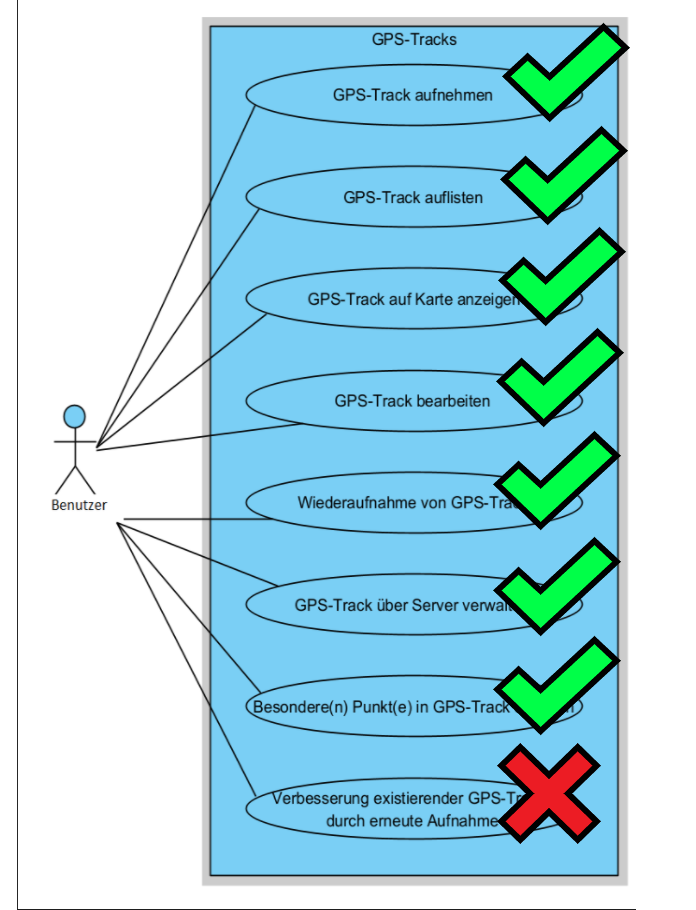
\includegraphics[scale=0.4]{use_case_comleted.png}
    \end{center}
    Während der Entwicklung wurde auch klar, dass die Verbindung der
    Anwendung mit dem Server gesichert werden musste. Derzeit kann jeder Benutzer einfach REST-Befehle verwenden, 
    um die GPS-Dateien auf dem Server zu ändern, zu löschen oder auch auf den Server
    herunterzuladen. Das ist eine schwerwiegende Sicherheitslücke, die bei missbräuchlicher Verwendung des APIs zu zahlreichen Problemen führen kann.
    \begin{center}
        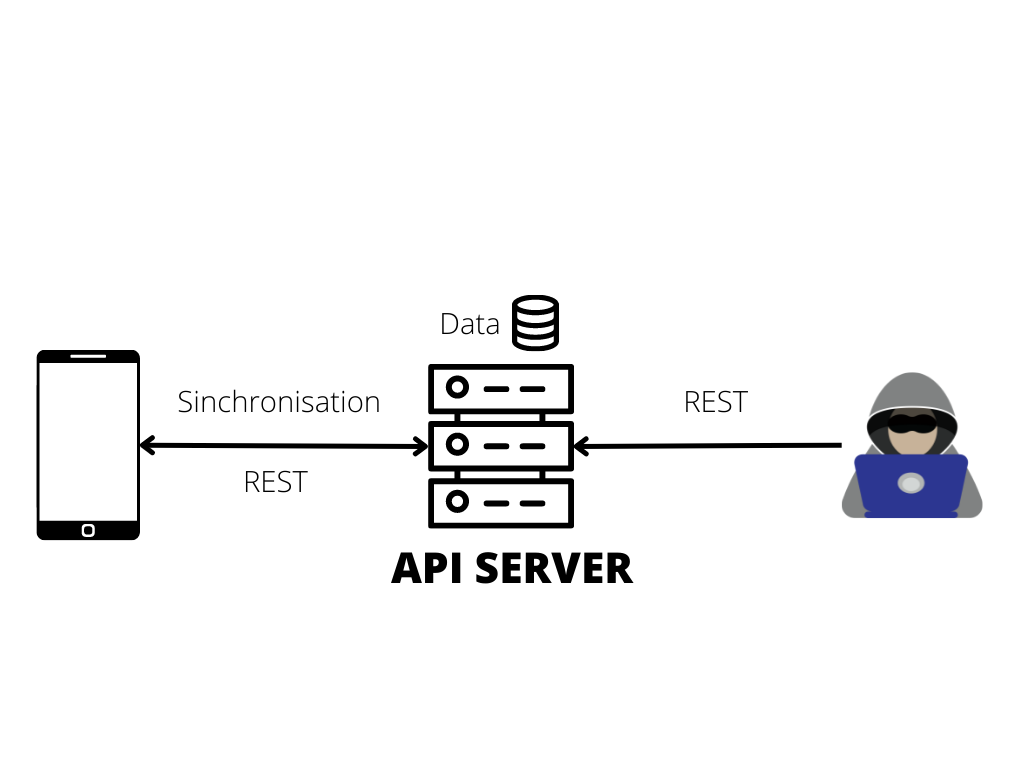
\includegraphics[scale=0.4]{Rest_API.png}
    \end{center}
    Aus diesem Grund sollte nächste logische Entwicklungsschritt
    daher der Authentifizierungs- und Autorisierungsprozess auf dem Server sein.
\subsection{Reflexion der Teammitglieder}
\subsubsection{Tom Nicolai}
    Ich war mit im Bereich der Programmierung der App zuständig. In den Meetings haben wir uns immer neue Features überlegt, 
    welche dann als GitHub Issues festgehalten wurden. Falls wir uns nicht während des Meetings einigen konnten, wer was macht, 
    hat sich jeder selbst das zugewiesen, worauf er grade Lust hatte. Auch haben wir unseren Zwischenstand immer mal wieder unserem 
    Auftraggeber Prof. Neugebauer gezeigt und uns Feedback dazu abgeholt. Somit konnten wir schnell sehen, ob etwas nicht so passt, 
    wie er es wollte. Die App selber haben wir in Java programmiert, was für mich gut war, da ich schon einige Erfahrung 
    in der Java Programmierung habe. Zwar habe ich noch nie eine Mobile App entwickelt, jedoch gewöhnte ich mich recht schnell 
    an die IDE und die neuen Bibliotheken. Programmiert habe ich immer nur alleine, jedoch habe ich mir auch ab und zu rat meiner 
    Teamkollegen eingeholt, bezüglich technischer Umsetzungen. Ein kleines Problem war noch, dass ich kein Android Handy besitze 
    und dementsprechend einige Features unserer App nicht ausprobieren konnte. Da wir untereinander jedoch gut vernetzt sind, 
    habe ich einfach mein neues Feature freigegeben und in unsere Gruppe geschrieben, ob es jemand testen könne. 
    Dort habe ich dann auch Feedback erhalten und konnte somit eventuelle Probleme direkt beheben. Alles in allem 
    war ich mit unserer Teamarbeit sehr zufrieden und bin mir sicher, dass wir ein gutes Produkt geschaffen haben.
\subsubsection{Aleksandr Pronin}
    Ich habe mein Team im Sommersemester kennengelernt. Zu diesem Zeitpunkt war die Android-App bereits teilweise fertig, 
    und wir mussten nur noch einen Plan für den Rest der Arbeit erstellen.
    Im ersten Schritt der Planung haben wir ein Verständnis geschaffen, wie wir die Rolle in unserem Team ungefähr verteilen können. 
    Meine Aufgabe war es, den Client-Server-Teil der Anwendung zu entwickeln und die entsprechende Dokumentation zu schreiben,
    da ich in diesem Bereich schnell und effektiv arbeiten kann.
    Das Domänenmodell, das zeigt, welche Elemente im initialen MVP vorkommen sind, wurde mir klar und ich hatte also eine gute Vorstellung
    davon, wie meine Arbeit ablaufen sollte.  Im Rahmen agile Vorgehensweisen sprachen wir ständig mit unserem Auftraggeber Prof. Neugebauer, 
    um die Anforderungen an die App zu konkretisieren und optimale Lösung konzipieren zu können. Mit all diesen Informationen konnten wir,
    technische Aspekte und Entwürfe zu User Interfaces zu erarbeiten. Wir haben außerdem beschlossen, einen wöchentlichen Daily zu führen, 
    um einen besseren Überblick über den Stand unseres Projekts zu erhalte. Ich denke, dass dies eine gute Technik ist, um im Team Gesamtergebnisse 
    zu erzielen. \\
    Bei dem Projekt, das meine Kollegen unterstütz und mitentwickelt haben, handelt es sich um eine Android-App zur 
    Speicherung von GPS-Routen und zum Austausch dieser Daten zwischen Geräten über einen Server. Application Server wurde
    in Python unter Verwendung des Flask-Frameworks geschrieben und die clientseitigen Komponenten wurden von mir 
    in Java weiterentwickelt. \\ Rückblickend kann ich sagen, dass wir im Rahmen der Gruppenarbeit sowie  gute Verständnis von agile 
    Entwickeln der App und insbesondere ein kompetentes Management besser erfassen konnten, als auch alle Besonderheiten der Entwicklung komplexer
    Softwaresysteme erkannt haben. Aus meiner Erfahrung als Werkstudent beim MMS T-Systems kann ich mit Zuversicht sagen,
    dass wir gemeinsam hervorragende Ergebnisse erzielt haben. Es hat Spaß gemacht, erfolgreich mit dem Team zusammenzuarbeiten und das Projekt zu 
    unterstützen. Dank meiner Kollegen(oder auch Kommilitonen) und unseres Projekts konnte ich jede Menge lernen.
\subsubsection{Alex Schechtel}
    Im zweisemestrigen Modul Software Engineering wurde ich zum ersten mal damit konfrontiert, ein erstes großes Softwareprojekt in einem Team umzusetzen.
    Größtenteils war ich im Projekt in der Implementierung der App tätig und beschäftigte mich mit dem Overlay der App und den Funktionen verschiedener Buttons.
    Ich hatte zuvor keine Erfahrung in der Appentwicklung und ko    nnte viele neue Dinge lernen.
    Dazu gehören die Gestaltung einer App und Zuweisung von Funktionen an die Buttons,
    aber auch wie man ein komplexes Softwaresystem plant und am besten umsetzt. 
    Da wir Java als Programmiersprache der App benutzten und ich schon Vorkenntnisse in Java besaß, 
    war es kein Problem sich an die Appentwicklungsumgebung zu gewöhnen.\\ 
    Ein Problem, welches ich bei der Entwicklung der App hatte, war es, den implementierten Code der Teammitglieder zu verstehen.
    Aber da wir über eine sehr gute Kommunikation verfügten, wurden diese Probleme sehr schnell aus dem Weg geschafft.
    Wenn ich mal Fragen oder Probleme bei der Entwicklung hatte wurde mir von den Teamkollegen immer geholfen.
    In den Meetings (im Team) herschte immer ein sehr lockeres und angenehmes Arbeitsklima, 
    was zusätzlich zu einer guten Gruppenarbeit beigetragen hat. \\
    Die Kommunikation mit dem Themensteller bereitete uns auch keine Probleme. Es konnte immer nach Anfrage ein Termin gefunden werden. 
    Alles in allem hat mir das Projekt viel Spaß gemacht, da ich jede Menge neue Dinge lernen konnte und ich denke, 
    dass wir gute Arbeit geleistet haben.
\subsubsection{Quang Duy Pham}
	Vor dem Besuch des Moduls Software Engineering hatte ich keine Erfahrung mit der Arbeit im Team oder in einem komplexen Projekt. Dies war eine große Herausforderung für mich zu meistern.Am Anfang habe ich mich für Tester und Entwurf entschieden. Als Entwurf habe ich einige Ideen zu Use-Cases und Struktur des Projekts gegeben, aber es gab keinen signifikanten Beitrag in Rolle Entwurf und hauptsächlich noch als a Tester.\par
	Obwohl ich den Quellcode nicht direkt implementiert habe, da mir die Programmiererfahrung fehlt. Ich muss immer noch den Quellcode und die Projektstruktur verstehen, um erfolgreiche Testfälle durchzuführen. Als Tester habe ich viel über Testmethoden und Dokumentationenbeschreibung gelernt. Außerdem habe ich einige kleine Beiträge gemacht, die nicht codierungsbezogen sind, wie Format der Dokumentationen prüfen, Mehrsprachenfunktion implementieren und kleine UI anpassen.\par
	Ich konnte Fehler jedoch nicht selbst beheben, weil ich Angst habe, dem Code kaputt zu machen, also bat ich oft andere Teamkollegen um Hilfe.\par
	Nach dem Modul Software Engineering hoffe ich, dass ich meine Kommunikation mit anderen verbessern konnte. Ich würde gerne mehr über das Programmieren lernen und beim nächsten Mal als Implementierung arbeiten. Schließlich möchte ich bessere Sprachkenntnisse haben, um bessere Dokumentationen schreiben zu können.\par
\subsubsection{Ludwig Schönthier}
    Ich habe von Beginn an, also seit dem Wintersemester 21/22 an dem Softwareprojekt mitgearbeitet. Für mich persönlich war das mein erstes Softwareprojekt,
    was aber nicht bedeutet, dass es keinen Spaß gemacht hat. In meiner Rolle als Analyst war ich hauptsächlich für die Dokumentation zuständig. Ich habe Protokolle
    erstellt, Use-Cases ausgearbeitet oder beispielweise Risiken bewertet. Leider hatte ich selbst bei kleinen Programmieraufgaben große Probleme, was meiner geringen
    Erfahrung zuzuschreiben ist. Daraufhin einigten wir uns, im Sinne der effektiveren Arbeit, mir keine Implementierungsaufgaben mehr anzuvertrauen aber im Gegenzug
    erledigte ich viel Dokumentationsarbeit.
    Im Großen und Ganzen hat mich die Zusammenarbeit in unserem Team sehr überzeugt. Bei Fragen stand einem das Team immer schnell zur Seite und auch bei Meetings
    arbeiteten wir alle diszipliniert aber auch in lockerer Atmosphäre und konnten unsere Arbeit somit effektiv abschließen. Die gute Gruppendynamik und geregelte
    Arbeitsteilung führten immer zu einer klaren Verteilung der Aufgaben und es traten keine signifikanten Probleme innerhalb des Teams auf. Zusätzlich konnten wir uns
    im Laufe der beiden Semester viele Fähigkeiten aneignen beziehungsweise diese verbessern, welche zur Entwicklung eines komplexeren Softwaresystems erforderlich sind.
        Letzten Endes bin ich sehr zufrieden mit dem Ausgang unseres Projektes und denke, jedes einzelne Teammitglied hat eine sehr gute Arbeit geleistet. Mir hat die
    Arbeit am Projekt auch sehr gefallen, da sie in einem äußerst angenehmen Umfeld geschah, was auf ein sehr kompetentes Team und gute Kommunikation mit Coach und
    Themensteller schließen lässt. In meinem nächsten Projekt werde ich auf jeden Fall versuchen, mehr Implementierungsarbeit zu leisten, um meine Kenntnisse und
    Expertise zu verbessern.

\subsubsection{Raphael Neubert}
Mit Team getriebener Projektarbeit im technologischen Bereich bin ich bereits vor dem Projekt in
Berührung gekommen. Während der 11. Klasse im Fachabi hatte ich 2 Tage pro
Woche, Praktika bei einem Start-up, was während meiner Zeit von einer Kooperation
übernommen wurde. In dieser Zeit konnte ich beobachten, wie sich die
eher lockeren agilen Methoden des Start-ups durch sehr strenge agile Methoden
der Kooperation ersetzt wurden. Des Weiteren hatte ich engen Kontakt sowohl
mit Entwicklern, als auch mit Projektleitern. Während meines Praktikums war ich allerdings
nicht in der Softwareentwicklung tätig. Außerdem wurden die agilen Aspekte der Projektarbeit hauptsächlich von
Projektleitung erledigt und so wusste ich zwar wie gute agile Zusammenarbeit aussieht, jedoch nicht wie sie wirklich
umgesetzt ist.\par
\medskip
Umso interessanter fand ich das Arbeiten an unserem eigenen Projekt. Ich hatte vor dem Projekt schon
Erfahrung mit Softwareentwicklung, aber noch nicht mit Softwareentwicklung im Team. Meine Erfahrungen mit der
Programmiersprache Java hielten sich in Grenzen und mit Android Entwicklung hatte ich überhaupt keine Erfahrung.
Mit Git hatte ich allerdings schon einige Erfahrung, weshalb ich auch in meinem Account das Repository erstellte
und verwaltete.\par
\medskip
Den Start des Projektes empfand ich persönlich als sehr chaotisch. Die fehlende Erfahrung war auf allen Ebenen
zu spüren. Dadurch wurden aber Verbesserungen noch viel deutlicher sichtbar, was mir sehr viel Motivation gegeben
hat. Nach den ersten Wochen stellte sich raus, dass ich mich mit den verschiedenen Technologien schon etwas besser auskannte
als die meisten. Ich wurde daher in Softwareengineering-I zur Schnittstelle zwischen dem Entwicklungsteam und den
Analysten sowie Wirtschaftsingenieuren. Ursprünglich hatte ich mich bereiterklärt, in Softwareengineering-II die
Projektleitung zu übernehmen. Als dann aber die Zeit kam, hatte ich die Sorge dadurch nicht mehr genügend Zeit
für die Entwicklung zu haben. Ich war sehr froh als Ludwig Schönthier sich bereiterklärte ebenfalls in der
Projektleitung mitzuwirken und so teilten wir uns die Projektleiteraufgaben auf. Ich übernahm dabei hauptsächlich
die Leitung der Entwicklung und Ludwig Schönthier stellte sicher, dass wir die ganzen Dinge um die Entwicklung
herum nicht aus den Augen verloren. Dadurch konnte ich mich sehr stark auf die Entwicklung fokussieren, was auch
sehr stark am Ergebnis zu sehen ist. Am Anfang von Softwareengineering-II hätte ich nicht gedacht, dass wir es
schaffen werden, mehr Funktionalität als das Aufnehmen und Bearbeiten der GPS-Tracks zu implementieren.
Dass wir es schaffen werden, fast alle Use-Cases zu implementieren, hätte ich zu diesem Zeitpunkt nicht geglaubt.
Dieser unerwartete Erfolg ist meiner Meinung nach das Resultat der ständigen Verbesserungen an unserer Arbeitsweise.\par
\medskip
Ich war im Projekt in allen Aspekten bis auf \say{Testing} involviert.
Dadurch habe ich enorm viel auf allen möglichen Ebenen gelernt. Besonders gut hat mir gefallen, dass wir
alle möglichen Dinge ausprobieren konnten. Diese Möglichkeit haben wir viel genutzt und so einige Dinge versucht,
gemerkt, dass sie sinnvoll sind und behalten, aber auch sehr häufig Dinge versucht und wieder verworfen, weil sie für
unser Projekt nicht bereichernd waren.
In der Berufswelt wird dieses herumprobieren so nicht möglich sein.\par
\medskip
Mit meinem Team war ich sehr zufrieden. Bis auf die Probleme mit Richard Michel, der uns aber nach Softwareengineering-I
verlassen hat, war unsere Zusammenarbeit sowie unsere Kommunikation sehr gut. Es gab in dem gesamten Projekt keinen
einzigen Streit. Trotz stressiger Belegarbeitszeit war es
immer möglich, Teammitglieder zur Erledigung wichtiger Aufgaben zu motivieren. Vor allem beeindruckt hat mich die
Offenheit meines Teams gegenüber meinen verrückten Ideen z. B. die Verwendung von Element statt Discord oder
das Schreiben des Projektberichts sowie der Anleitungen in LaTeX.\par 
\medskip 
Insgesamt bin ich mit dem Projekt sehr zufrieden und möchte mich bei Ihnen und bei meinem Team bedanken.
\end{document}

\subcection{Anhänge}
Iterationspläne:
\include{}
Iterationsplan 3
\include
Iterationsplan 4
\include
Iterationsplan 5
\include
Iterationsplan 6
\include
Iterationsplan 7
\include
Iterationsplan 8